\section{Methodology}
% \addcontentsline{toc}{section}{Methodology}
\fancyhead[R]{Methodology}

\subsection{Data Collection}
\label{sec:Data Collection}

Data collection is a crucial step in model building, as the quality and relevance of the data directly impact the model’s performance.. The data for this thesis was collected from UniProt, a comprehensive resource that provides detailed protein sequence and functional information. UniProt or Universal Protein Resource is a central protein sequence, and annotation database. It is widely accepted as comprehensive and provides high-quality data, which makes it a must to perform bioinformatics and computational biology. UniProt pools in much valuable information: experimental findings, different kinds of analyses, and literature information and hence provides rich and reliable sources of further research. Researchers can receive high-quality reviewed entries with 3D structural data and catalytic properties in place, which makes the data reliable and applicable for predicting enzyme functions. \autocite{uniprotconsortiumUniProtUniversalProtein2021}

Some of the main features of UniProt are:

\begin{itemize}
    \item \textbf{Comprehensive Protein Data:} UniProt contains a vast collection of protein sequences, functional annotations, and cross-references to other databases, making it a valuable resource for protein research.
    \item \textbf{Reviewed Entries:} UniProt contains both reviewed (Swiss-Prot) and unreviewed (TrEMBL) entries. Reviewed entries are manually curated by experts, ensuring high accuracy and reliability.
    \item \textbf{Functional Annotations:} Each protein entry includes detailed functional annotations, such as catalytic activity, biological processes, and involvement in pathways.
    \item \textbf{3D Structural Data:} UniProt links to structural databases like PDB, providing access to 3D structures of proteins, which are crucial for understanding enzyme mechanisms.
    \item \textbf{Cross-references:} Extensive cross-references to other databases (e.g., PDB, BRENDA, Reactome) enhance the richness of the data.
\end{itemize}

For this study, UniProt was chosen due to its high-quality data, extensive coverage of protein information, and user-friendly interface. The data collection process involved querying UniProt for enzyme entries with 3D structural data and catalytic activity annotations, extracting relevant information, and preprocessing the data for model development. The data retrieval process utilized the UniProt REST API to download protein data that met specific criteria. The criteria included reviewed entries with both 3D structural data and catalytic properties. A figure of the data collection and processing workflow is shown in the appendix \ref{fig:Data-Preparation-Processing-Workflow}.

\begin{compactenum}
    \item API Request: The script constructs a query to the UniProt REST API to retrieve reviewed protein entries with specified fields and criteria.
    \item Data Retrieval: Data is retrieved and transformed into a pandas DataFrame for further processing.
    \item Data Filtering: The DataFrame is filtered to retain entries with non-null EC numbers and PDB codes.
    \item PDB Download: The PDB files corresponding to the protein entries are downloaded from the PDB database using the PDB IDs.
\end{compactenum}

\subsection{Data Preprocessing}
\label{sec:Data Preprocessing}

After the data collection, the next step is to preprocess the data to make it suitable for model training. Data preprocessing involves several critical steps to prepare the dataset for the prediction model. These steps include data retrieval, cleaning, transformation, integration, and normalization. The goal of data preprocessing is to ensure that the data is clean, consistent, and suitable for training the model.

After collecting the sequences for every enzyme based on the Ligand-Binding-Site prediction, the sequences are cleaned by removing any non-standard amino acids, special characters, or gaps. These types of amino acids can not be processed by the model and need to be removed. These could for example be "B", "J", "O", "U", "X", or "Z".  This step ensures that the sequences contain only valid amino acid residues, which is crucial for accurate modeling. \autocite{OneletterNotationAmino1972}

The cleaned sequences are then tokenized and encoded into numerical data for input into the model. This involves converting each amino acid into a unique integer identifier. The sequences are also padded to ensure they all have the same length, which is necessary for batch processing in Deep Learning models. Tokenization and padding allow the model to handle sequences of varying lengths and ensure uniform input size for the neural network. \autocite{dangRepeatedPaddingData2024}

For gaining a first insight into the dataset, the distribution of EC classes in the dataset was analyzed. The table indicates that the dataset is highly imbalanced, with Transferases being the most common class and Ligases the least common. This imbalance can affect the model's performance, as it may struggle to learn from underrepresented classes.

\begin{table}[!htbp]
    \centering
    \begin{tabular}{lrr}
        \toprule
        EC Class & Count \\
        \midrule
        Oxidoreductases & 23544 \\
        Transferases & 59022 \\
        Hydrolases & 41283 \\
        Lyases & 2376 \\
        Isomerases & 4617 \\
        Ligases & 1323 \\
        Translocases & 1836 \\
        \bottomrule
    \end{tabular}
    \caption{Distribution of EC classes in the dataset}
    \label{tab:ec-class-distribution}
\end{table}

To address this issue, the dataset was balanced using the RandomUnderSampler algorithm from the imbalanced-learn library. The RandomUnderSampler uses a sampling strategy with k=2500 to balance the dataset by selecting ec classes that have more than 2500 samples. This approach ensures that the model is trained on a more balanced dataset, which can improve its performance on underrepresented classes. The following comparison shows the distribution of EC classes before and after balancing the dataset:

\begin{figure}[!htbp]
    \centering
    \begin{minipage}[t]{\textwidth}
    \caption{Distribution of EC classes before and after balancing}
    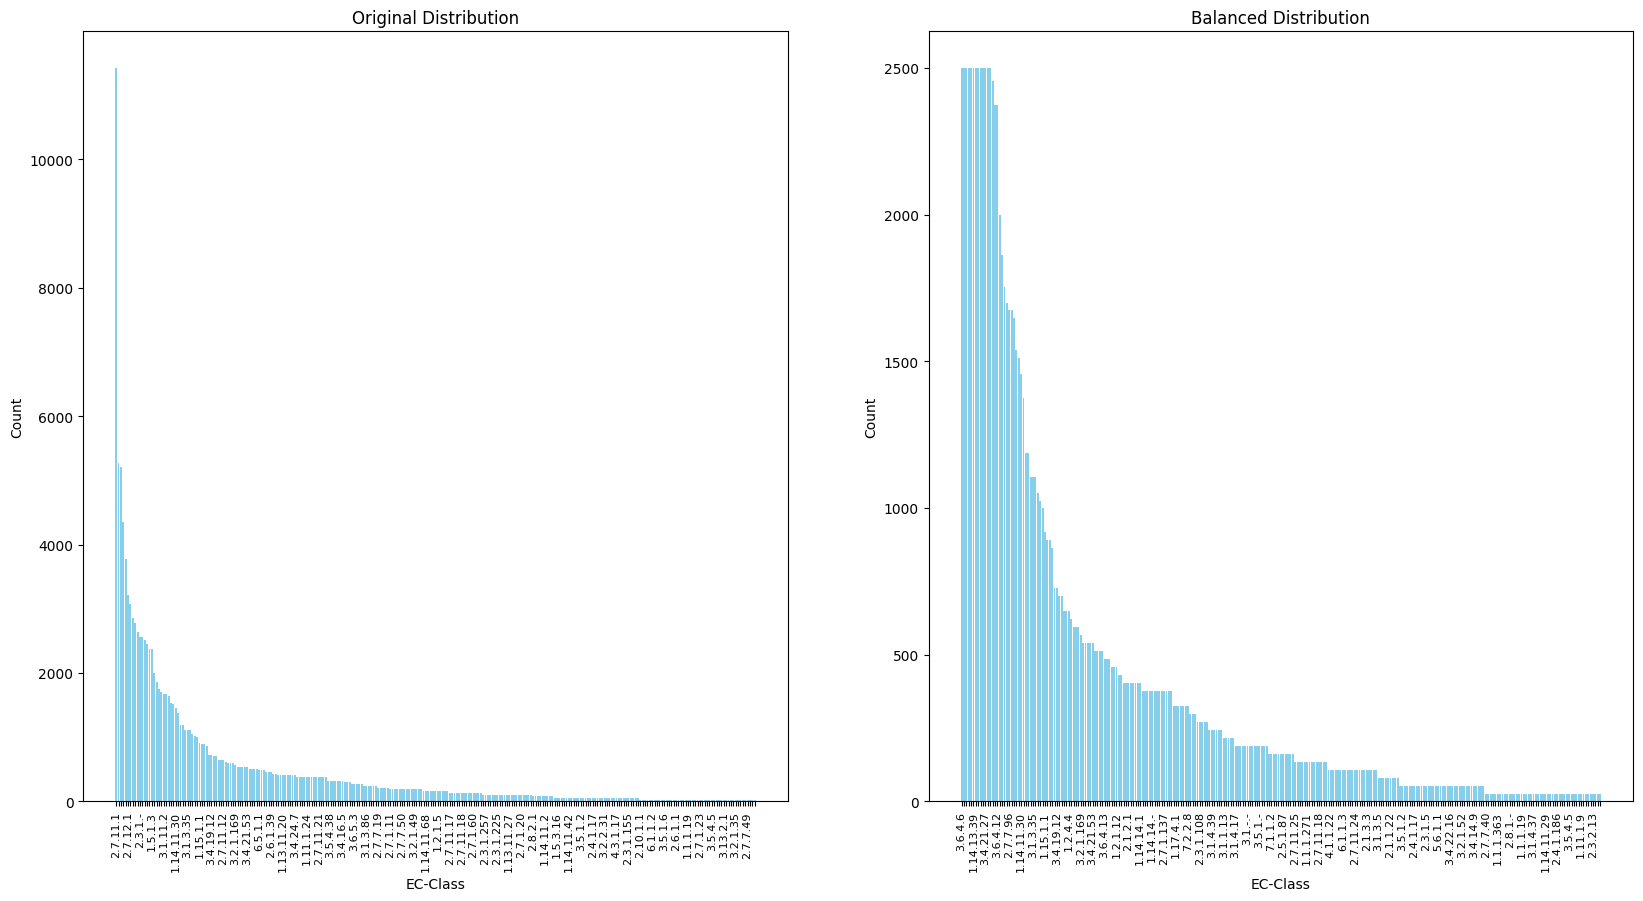
\includegraphics[width=1\textwidth]{img/ec-distribution-comparison.png}
    \source{Own illustration}
    \label{fig:ec-distribution-comparison}
    \end{minipage}
\end{figure}

Taking a closer look at the distribution of EC classes on the second level of the hierarchy, the class 2.7 (Phosphotransferases) is the most common, while the class 2.6 (Acyltransferases) is the least common. This is because Phosphotransferases are involved in a wide range of cellular processes, making them more prevalent in the dataset. The class 2.6, on the other hand, is more specialized and less common in the dataset. After rebalancing the dataset, the distribution of EC classes is more uniform, but still not perfectly balanced. To keep the original distribution of the dataset, the distribution was kept as it is. Further optimization may be required, but is beyond the scope of this study and would require additional data in the UniProt database.

Finally, the transformed features are integrated into a single dataset. The data is then normalized to ensure that all features are on a similar scale, which is important for the convergence of Deep Learning models. Normalization helps in speeding up the training process and achieving better performance. \autocite{ioffeBatchNormalizationAccelerating2015}

\subsection{Feature Engineering}
\label{sec:Feature Engineering}

Feature engineering is a critical step in preparing data for prediction models. This process involves transforming raw data into meaningful features that can improve the performance of the model. To capture meaningful information from protein sequences, this study used several features derived from the sequences, including amino acid composition, molecular weight, isoelectric point, hydrophobicity, and sequence length. These features provide valuable insights into the physicochemical properties of the proteins, enabling the model to learn patterns that correlate with enzyme functions. The ProteinAnalysis class from the Biopython library was used to calculate these features.

Amino acid composition refers to the relative frequency of each of the 20 standard amino acids in a protein sequence. Proteins are made up of amino acids, which are the building blocks that determine the protein's structure and function. Each amino acid has unique properties that influence the protein's overall characteristics. \autocite{ProteinStructureLearn}

The amino acid composition provides information about the protein's primary structure, which is essential for understanding its function. The amino acid composition is calculated as the percentage of each amino acid in the sequence. For example, a protein with a high proportion of hydrophobic amino acids may be in ec class 2.1 (Transferases), because these enzymes often have hydrophobic binding sites. \autocite{lightTransferaseHydrolaseRole2017}

Molecular weight is the total mass of all the amino acids in a protein sequence. It is measured in Daltons (Da) and reflects the size of the protein. The molecular weight of a protein influences its physical and chemical properties, such as solubility and interaction with other molecules. Larger proteins may have more complex structures with multiple functional domains, which can affect their enzymatic activity.

The isoelectric point (pI) is the pH at which a protein carries no net electrical charge. At this pH, the number of positive and negative charges on the protein is equal, resulting in minimal solubility. The pI of a protein affects its solubility and interaction with other molecules. Proteins are least soluble at their pI and more likely to precipitate. This property is important for understanding protein behavior in different pH environments, which can influence their function and stability. By including pI as a feature, the model can better predict how proteins will behave in various conditions, aiding in accurate enzyme classification.

Hydrophobicity, measured by the Grand Average of Hydropathy (GRAVY) score, indicates the overall hydrophobic or hydrophilic nature of a protein. It is calculated by averaging the hydropathy values of all amino acids in the sequence. Hydrophobicity affects protein folding, stability, and interaction with membranes. Proteins with high hydrophobicity are likely to be involved in membrane-related processes, while those with low hydrophobicity are generally more soluble in water. Understanding the hydrophobic or hydrophilic nature of a protein is crucial for predicting its function, especially in relation to its interaction with other molecules and environments. \autocite{khosraviIdentificationCharacterizationInulinases2023}

These biochemical features provide a multi-dimensional representation of protein sequences, capturing both sequence-specific information and physicochemical properties. By integrating these features, the model gains a comprehensive understanding of the proteins, enabling more accurate and reliable predictions. The features were chosen in a comprehensive analysis and are also based on a study by Gainza et al. (2020), which highlights the importance of incorporating these specific physicochemical features in protein function prediction models. \autocite{gainzaDecipheringInteractionFingerprints2020}

\pagebreak
\subsection{Model Architecture}
\label{sec:Model Architecture}

The model architecture is a critical component of the prediction process, as it determines how the data is processed and transformed to make predictions. This study's model architecture is designed to leverage both raw protein sequences and biochemical features to accurately predict enzyme classes. The model architecture is shown in the figure below:

\begin{figure}[hbt]
    \centering
    \begin{minipage}[t]{\textwidth}
    \caption{Model Architecture}
    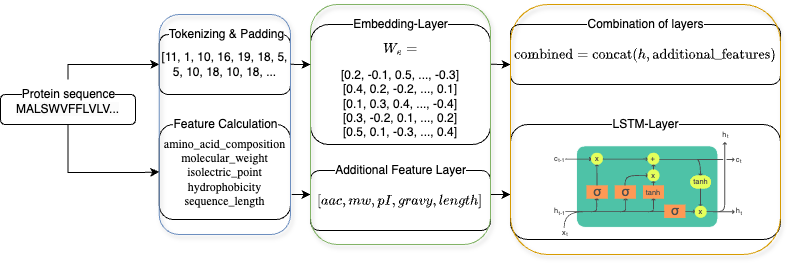
\includegraphics[width=1\textwidth]{img/Model-Architecture.drawio.png}
    \source{Own illustration}
    \label{fig:model-architecture}
    \end{minipage}
\end{figure}

To integrate raw protein sequences into the model, the sequences are first tokenized and passed through an embedding layer. Each amino acid is mapped to a unique integer. For example, the sequence "ACDEFGHIKLMNPQRSTVWY" is tokenized into a list of integers. This process can be mathematically represented as:

\begin{equation}
    token(x) = i \ \text{where}\ x \in \{A, C, D, E, F, G, H, I, K, L, M, N, P, Q, R, S, T, V, W, Y\} \\
\end{equation}
and $i$ is the index of amino acid $x$ in the list.

The tokenized sequence is then passed through an embedding layer that transforms these integers into dense vectors, capturing the contextual meaning of each amino acid within the sequence. This embedding process is essential for understanding the relationships between amino acids and their roles in protein function.

\begin{equation}
    \text{embedding}(i) = v
\end{equation}
where $v_i$ is the embedding vector for the token $i$.

These embeddings are fed into the Recurrent Neural Network (RNN), which processes the sequence and updates its hidden states accordingly, allowing the model to capture complex dependencies and interactions between amino acids. Sequences are then padded to ensure they all have the same length, necessary for batch processing in deep learning models.

Integrating raw protein sequences as a separate layer in the model allows for the extraction of complex patterns and dependencies within the sequences, similar to how large language models (LLMs) like ProtBERT process natural language. ProtBERT, a pre-trained language model for protein sequences, demonstrates the effectiveness of using raw sequence data for protein function prediction by capturing intricate patterns and dependencies. By integrating raw sequences, the model benefits from advanced sequence modeling capabilities, improving its predictive performance. \autocite{brandesProteinBERTUniversalDeeplearning2022}

Using techniques similar to those employed in LLMs, the model captures contextual relationships between amino acids, enhancing its ability to predict enzyme functions. This approach is particularly useful for understanding long-range interactions and dependencies that are crucial for protein function.

Biochemical features such as molecular weight, isoelectric point, hydrophobicity, and sequence length provide additional context that can enhance prediction accuracy. These features help the model understand the physical and chemical characteristics of the proteins, which are critical for predicting enzyme functions.

\begin{enumerate}
    \item \textbf{Embedding Layer:} Converts amino acid sequences into dense vector representations, capturing semantic similarities between amino acids. This layer allows the model to handle varying sequence lengths and learn useful representations of amino acids in the context of their sequence.
    \item \textbf{LSTM Layers:} Long Short-Term Memory (LSTM) layers capture long-range dependencies in the sequence data, which is crucial for understanding the functional context of amino acids within the sequence. LSTMs are particularly effective in modeling sequential data due to their ability to remember information for long periods and manage the vanishing gradient problem. Studies have demonstrated the effectiveness of LSTMs in various sequence analysis tasks, including protein function prediction. \autocite{liuAttentionMechanismEnhanced2019}
    \item \textbf{Concatenation Layer:} Combines the output of the LSTM layers with the additional biochemical features, allowing the model to leverage both sequence-based and property-based information. This integration ensures that the model considers both the sequence context and the biochemical properties of the proteins.
    \item \textbf{Dense Layers:} Integrates the combined features and produce the final classification output. These layers apply non-linear transformations to the combined features, enabling the model to learn complex patterns and relationships. The dense layers are responsible for making the final predictions based on the input data, providing the model's output for each EC class.
\end{enumerate}

To address the hierarchical nature of the Enzyme Commission (EC) classification system, the data is split into four levels of the EC hierarchy. The first level represents the broadest classification, while the fourth level provides the most specific classification. This ensures that models are trained and evaluated on appropriately structured data, allowing for predictions at varying levels of specificity. Each level of the hierarchy requires a different degree of detail and understanding, and splitting the data accordingly helps tailor the model's learning process to the complexity of each classification level.

The integration of both sequence-based features and biochemical properties provides a comprehensive and multi-dimensional representation of proteins, enhancing the model's ability to make accurate and reliable predictions of enzyme classes. This holistic approach ensures that the model leverages the strengths of detailed biochemical properties and advanced sequence modeling, resulting in a robust and effective predictive tool.